\documentclass[11pt,a4paper]{article}
\usepackage[utf8]{inputenc}\usepackage[T1]{fontenc}
\usepackage[provide=*,ngerman]{babel}
\usepackage{lmodern,microtype,amsmath,amssymb,booktabs,tabularx,array,xcolor,fancyhdr,geometry,graphicx,hyperref}
\geometry{left=20mm,right=20mm,top=20mm,bottom=21mm}
\definecolor{ink}{HTML}{173643}\definecolor{teal}{HTML}{08786F}\definecolor{muted}{HTML}{53636B}\definecolor{pale}{HTML}{EFF6F5}
\hypersetup{colorlinks=true,urlcolor=teal,linkcolor=teal,pdftitle={CST Staubball: Unabhaengige Bounce-Vorhersage v0.1},pdfauthor={X6 Astrolabium Arbeitsdokument}}
\pagestyle{fancy}\fancyhf{}\fancyfoot[L]{\small\sffamily\color{muted}X6 Astrolabium · Bounce-Vorhersage v0.1}\fancyfoot[R]{\small\thepage/6}\renewcommand{\headrulewidth}{0pt}
\setlength{\parindent}{0pt}\setlength{\parskip}{5pt}\setlength{\emergencystretch}{2em}
\newcolumntype{Y}{>{\raggedright\arraybackslash}X}
\newcommand{\kicker}[1]{{\sffamily\small\bfseries\color{teal}#1}\par}
\newcommand{\tit}[1]{{\sffamily\LARGE\bfseries\color{ink}#1}\par\vspace{6pt}}
\newcommand{\sect}[1]{\par\vspace{6pt}{\sffamily\large\bfseries\color{ink}#1}\par}
\newcommand{\note}[1]{\par\vspace{4pt}\colorbox{pale}{\parbox{\dimexpr\linewidth-2\fboxsep}{#1}}\par}
\begin{document}
\kicker{FORSCHUNGSPRÜFUNG · 5. NOVEMBER 2026}
\tit{Eine Bounce-Vorhersage\\an neuen Anfangszuständen prüfen}
\textbf{Die frühe Vorhersage besteht den Test im reduzierten Referenzmodell. Ein eigenständiger CST-Bounce und Singularitätsauflösung sind damit nicht bestätigt.}

Aus zehn vorher festgelegten neuen Anfangszuständen wurden Zeitpunkt und Minimalwert des mittleren Volumens berechnet. Diese Prognosen wurden gespeichert und mit einer Prüfsumme fixiert, bevor eine getrennte numerische Zeitentwicklung die späten Daten erzeugte. Auf dem feinsten Gitter bestehen alle zehn Fälle die vorab gesetzten Grenzen: höchstens 1\,\% Zeitfehler und 3\,\% Volumenfehler.

\sect{Drei getrennte Entscheidungen}
\begin{tabularx}{\linewidth}{@{}>{\raggedright\arraybackslash}p{46mm}Y@{}}\toprule
\textbf{Prüffrage} & \textbf{Befund}\\\midrule
Vorhersage eines Minimums von $\langle V\rangle$ & \textbf{PASS im Referenzmodell.} Maximal 0,615\,\% Fehler im Zeitpunkt und 1,324\,\% im Minimalvolumen; beide Fehler sinken bei jeder der zwei Verfeinerungen.\\
Singularitätsauflösung & \textbf{Nicht nachgewiesen.} Bei allen acht geprüften Gaußzuständen divergiert $\langle V^{-2}\rangle$ am vorhergesagten Minimum. Diese Observable wird nicht mit einem Krümmungsoperator gleichgesetzt.\\
Unabhängige physikalische CST-Prognose & \textbf{HOLD / nicht prüfbereit.} Der vollständige gekoppelte CST-Kern und sein klassischer Grenzfall fehlen weiterhin. Die alte Ablehnung des dominanten Bounce-Kandidaten bleibt bestehen.\\\bottomrule
\end{tabularx}

\sect{Was hier unabhängig ist}
Die zehn Präparationen wurden im vorherigen Klassiktest [2] nicht verwendet. Die Prognose nutzt ausschließlich Anfangsmomente. Der spätere Löser erhält nur Anfangszustand, Hamiltonoperator und Gitter; er liest weder die prognostizierte Bounce-Zeit noch die Momentformel. Er entwickelt die Wellenfunktion mit einem räumlichen Differenzenoperator und Crank--Nicolson. Das späte Minimum wird aus den erzeugten Ablesewerten bestimmt.

Es handelt sich um eine \textbf{getrennte rechnerische Gegenprüfung mit neuen synthetischen Eingaben}. Es ist keine unabhängige physikalische Messung, keine Replikation durch eine andere Forschungsgruppe und keine externe Präregistrierung. Beide Rechnungen prüfen dieselbe ausdrücklich angenommene reduzierte Dynamik.

\note{\textbf{Begriff des Bounce in diesem Test:} ein striktes inneres Minimum des Erwartungswerts $\langle V(T)\rangle$ mit vorheriger Abnahme und anschließender Zunahme. Das ist keine Wahrscheinlichkeit einer mehrzeitigen Bounce-Historie und kein erneuter Test der alten 80-\%-Dominanzforderung.}

\newpage
\kicker{01 · PROGNOSE AUS FRÜHEN DATEN}
\tit{Drei Anfangsmomente genügen im Modell}
Wir verwenden unverändert die homogene flache periodische Staubreferenz, $q=\sqrt V>0$, $\kappa=3\pi G/2$, $H=-\kappa p^2$ und den gewählten Dirichlet-Rand $\psi(0)=0$. Die direkte $q$-Quantisierung verwendet $dq$. Für die folgenden numerischen Werte gilt dimensionslos $\kappa=1$. Es gibt weder einen Staubballrand noch einen Außenraum.

Seien für den normierten Anfangszustand
\[
 A=\langle q^2\rangle_0,\quad
 J=2\hbar\int_0^\infty q\,\operatorname{Im}(\overline\psi_0\psi'_0)\,dq,
 \quad E=\hbar^2\int_0^\infty|\psi'_0|^2\,dq.
\]
Die ungerade Fortsetzung auf die volle Gerade entwickelt sich frei. Dort gilt $q(T)=q-2\kappa pT$; die geraden Momente stimmen mit denen der Halbgeraden überein. Daher exakt
\[
 \langle V(T)\rangle=A-2\kappa JT+4\kappa^2ET^2,
 \qquad \boxed{T_b=\frac{J}{4\kappa E},\quad V_b=A-\frac{J^2}{4E}}.
\]
Für $J>0$ liegt das Minimum in der Zukunft. Die normierte ungerade Fortsetzung hat verschwindende volle Orts- und Impulsmittelwerte. Die Robertson--Schrödinger-Ungleichung liefert $AE-J^2/4\ge\hbar^2/4$, somit
\[
 V_b\ge\frac{\hbar^2}{4E}>0,\qquad \overline M=\kappa E.
\]
Dies ist eine strukturelle Eigenschaft dieses Operators, seiner Randwahl und Zustandsklasse. Sie ist keine neue, aus der CST-Summe hergeleitete Abstoßung. Die Schranke liefert keine von $\hbar$ unabhängige Mindestgröße.

\sect{Vorher festgelegte neue Präparationen}
Mit $g_{Q,P,s}(q)=(2\pi s^2)^{-1/4}\exp[-(q-Q)^2/(4s^2)+iP(q-Q)/\hbar]$ setzen wir
\[
 f(q)=\sum_r c_r e^{i\theta_r}g_{Q_r,P_r,s}(q),\qquad
 \psi_0(q)=\frac{f(q)-f(-q)}{\|f-f(-\cdot)\|_{q>0}}.
\]
G01--G08 sind alle acht Kombinationen $Q\in\{3,5\}$, $P\in\{0{,}7,1{,}3\}$, $\hbar\in\{0{,}03,0{,}06\}$ mit $s=0{,}25$ und $c=1$, $\theta=0$, in dieser Reihenfolge sortiert.

C01 ist eine kohärente Überlagerung mit $(Q,P,c,\theta)=(3{,}4,1,1,0)$ und $(4{,}6,1,0{,}6,\pi/3)$, $s=0{,}25$, $\hbar=0{,}03$. C02 benutzt $(3,0{,}8,1,0)$ und $(4{,}2,1{,}2,0{,}8,\pi/2)$, $s=0{,}30$, $\hbar=0{,}06$.

Alle zehn Zustände sind normiert, haben endliche kinetische Energie und kontrahierende frühe Volumenmittelwerte. Die genaue Energie und damit mittlere Staubmasse werden aus dem Zustand berechnet; der zentrale Impuls wird nicht als scharfe Masse behandelt.

\newpage
\kicker{02 · ERGEBNISSE DER SPÄTEN GEGENRECHNUNG}
\tit{Zehn Prognosen, drei Auflösungen}
Die separat gespeicherte Prognose \texttt{forecast.json} enthält keine späten Daten. Ihre SHA-256 beginnt mit \texttt{5dfe93f19732f2ca}. Die Anfangsintegrale wurden durch adaptive Quadratur ausgewertet. Plan und Prognose bleiben während der späten Rechnungen unverändert.

\begin{tabularx}{\linewidth}{@{}l r r r r@{}}\toprule
\textbf{Fall} & \textbf{$T_b$ prognostiziert} & \textbf{$V_b$ prognostiziert} & \textbf{Zeitfehler \%} & \textbf{Vol.-Fehler \%}\\\midrule
G01 & 2.127229 & 0.128140 & 0.157 & 0.325 \\
G02 & 2.081681 & 0.319439 & 0.046 & 0.127 \\
G03 & 1.151393 & 0.081631 & 0.615 & 0.675 \\
G04 & 1.144098 & 0.138538 & 0.162 & 0.400 \\
G05 & 3.545381 & 0.244834 & 0.157 & 0.473 \\
G06 & 3.469469 & 0.776219 & 0.046 & 0.145 \\
G07 & 1.918989 & 0.115641 & 0.615 & 1.323 \\
G08 & 1.906829 & 0.273718 & 0.162 & 0.562 \\
C01 & 1.866405 & 0.398906 & 0.331 & 0.204 \\
C02 & 1.779833 & 0.204231 & 0.101 & 0.324 \\
\bottomrule\end{tabularx}
{\small Fehler gegenüber der frühen Vorhersage, jeweils auf dem feinsten Gitter. Alle Werte sind dimensionslos.}

\sect{Vorab gesetzter numerischer Prüfvertrag}
Die Entwicklung läuft auf $0<q<32$ bis $T=6$ mit Dirichlet-Enden. Abgelesen wird stets alle 0,025 Zeiteinheiten. Das globale innere Gitterminimum und seine beiden Nachbarn bestimmen durch lokale Parabelinterpolation den beobachteten Zeitpunkt und Minimalwert. Die Vorhersage wird dabei nicht als Suchzentrum oder Fitvorgabe benutzt.

\begin{tabularx}{\linewidth}{@{}r r r r@{}}\toprule
\textbf{Raumpunkte} & \textbf{Zeitschritt} & \textbf{max. Zeitfehler \%} & \textbf{max. Vol.-Fehler \%}\\\midrule
2048 & 0,00500 & 10,230 & 18,467\\
4096 & 0,00250 & 2,478 & 5,150\\
8192 & 0,00125 & 0,615 & 1,324\\\bottomrule
\end{tabularx}

Gefordert wurden auf dem feinsten Gitter höchstens 1\,\% Zeitfehler, 3\,\% Volumenfehler, ein striktes inneres Minimum und abnehmende Fehler auf allen drei Auflösungen. Jeder Fall erfüllt diese Kriterien. Die größte Normabweichung über alle Läufe beträgt $1{,}88\cdot10^{-12}$; erlaubt waren $10^{-9}$.

\sect{Zusätzliche Kontrolle des Kontinuumskerns}
Eine separate Sinusentwicklung prüft alle zehn Zustände an jeweils fünf Zeiten gegen die Momentprognose. Der maximale Volumenfehler dieser 50 Kontrollen beträgt $3{,}56\cdot10^{-13}$. Damit wird die größere Abweichung der Differenzenrechnung als numerischer Fehler identifiziert. Die grobe Auflösung erfüllt die engen Endtoleranzen nicht; ihre Abweichung wird vollständig ausgewiesen.

Das sind Gleitkommaprüfungen mit festgelegten Toleranzen, keine rigorosen Intervallzertifikate. Raum- und Zeitauflösung werden gemeinsam verfeinert; ihre Fehleranteile wurden nicht separat bestimmt.

\newpage
\kicker{03 · WAS DIE UMKEHR IDENTIFIZIEREN KANN}
\tit{Ein Volumenminimum entscheidet noch nicht die Physik}
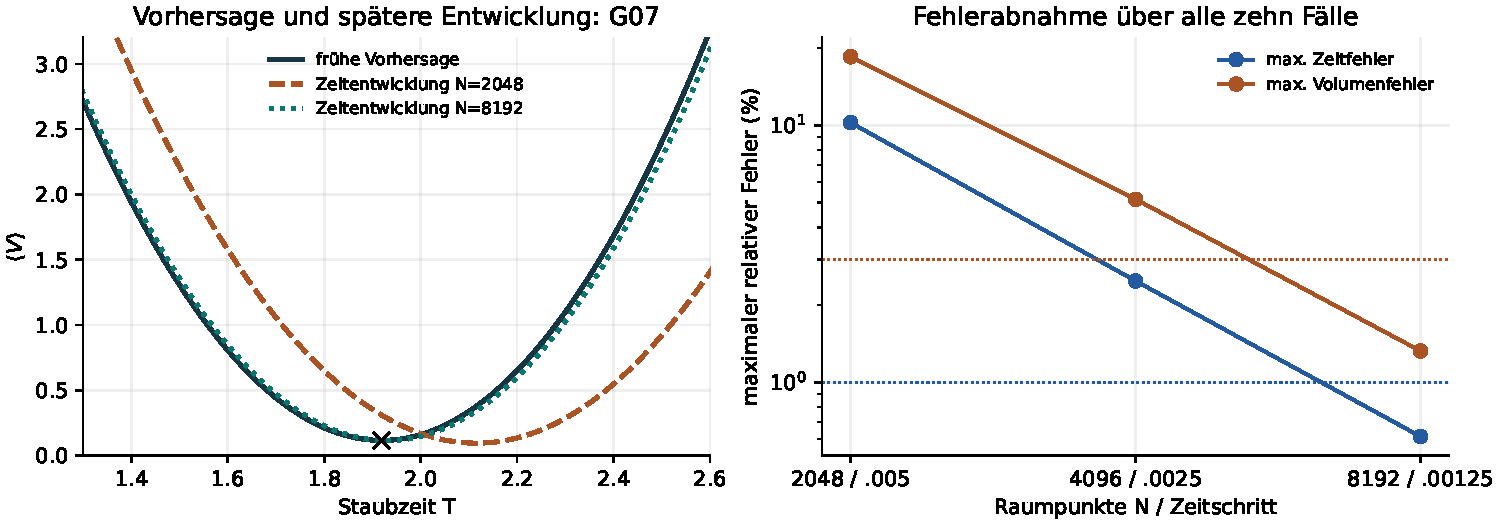
\includegraphics[width=\linewidth]{figures/prediction_test.pdf}\par
{\small\color{muted}Links: Die frühen Momente sagen die Kurve voraus; die getrennte Differenzenentwicklung nähert sich ihr bei Verfeinerung. Rechts: maximale Fehler über alle zehn Fälle. Gepunktete Linien markieren die vorab gesetzten Endtoleranzen.\par}

\sect{Dirichlet und Neumann}
Für G01 und G08 wurde zusätzlich die gerade Bildkombination $f(q)+f(-q)$ mit Neumann-Rand $\psi'(0)=0$ betrachtet. Auch sie besitzt eine unitäre Halbgeradenentwicklung. Ihre frühen Momente ergeben innerhalb der ausgeführten Gleitkommarechnung dieselben Werte von $T_b$ und $V_b$ wie Dirichlet; die Unterschiede der hier weit vom Rand präparierten Anfangspakete sind exponentiell klein. Eine direkte spätere Quadratur der Neumann-Bildlösung kontrolliert die Volumenprognose an jeweils drei Zeiten.

Die Wellenfunktion am Rand ist jedoch verschieden: Dirichlet erzwingt dort null; Neumann ergibt am vorhergesagten Minimum die Wahrscheinlichkeitsdichten 4,458 für G01 und 3,050 für G08. Das gemeinsame Volumenminimum identifiziert somit die Randphysik nicht. Die Kontrolle betrifft genau diese beiden Erweiterungen, nicht alle möglichen Robin-Ränder.

\sect{Kontrolle ohne reflektierende Wand}
Ein einzelnes Gaußpaket G01 auf der \emph{vollen} $q$-Geraden besitzt ebenfalls ein positives Minimum von $\langle q^2\rangle$, mit $T_b=2{,}127229$ und $V_b=0{,}128140$. Dabei läuft sein Schwerpunkt durch $q=0$ ins Negative. Bei $T=4{,}285714$ gilt $\langle q\rangle=-3$ und $P(q>0)\simeq7{,}76\cdot10^{-8}$; es ist nicht reflektiert worden.

Negative $q$ sind außerhalb der physikalischen Halbgeradenreferenz. Dies ist deshalb eine \textbf{diagnostische Gegenkontrolle}, kein alternatives physikalisches Staubmodell. Sie zeigt präzise, warum eine Umkehr von $\langle q^2\rangle$ allein nicht einmal Reflexion von einer bloßen Vorzeichenänderung unterscheiden kann.

\note{Die Vorhersage gilt für ein Volumenmittel. Weder einzelne Geometriehistorien noch ihre Dekohärenz oder eine Durchgangswahrscheinlichkeit sind damit bestimmt. Die alte Bounce-Ereignisfrage darf nicht durch dieses leichter erfüllbare Kriterium ersetzt werden.}

\newpage
\kicker{04 · REGULARITÄT AM VORHERGESAGTEN MINIMUM}
\tit{Positives Mittelvolumen ist keine Singularitätsauflösung}
Für einen einzelnen Gaußzustand sei $D=1-i\kappa\hbar T/s^2$ und $f_T$ seine freie volle Geradenlösung. Die normierte Dirichlet-Bildlösung hat nahe dem Rand die Entwicklung
\[
 \psi_D(q,T)=c(T)q+O(q^3),\qquad
 c(T)=\frac{2f_T(0)}{\mathcal N D}
       \left(\frac{Q}{2s^2}+\frac{iP}{\hbar}\right).
\]
$\mathcal N$ ist die positive Anfangsnorm. Für $Q>0$, endliches $s,\hbar>0$ und reelles $T$ ist $f_T(0)\ne0$, $D\ne0$ und die Klammer ungleich null. Also $c(T)\ne0$ zu jeder endlichen Zeit, insbesondere beim vorhergesagten Bounce. Daraus folgt
\[
 \int_\epsilon^\infty\frac{|\psi_D(q,T)|^2}{q^4}\,dq
   =\frac{|c(T)|^2}{\epsilon}+O(1),\qquad
 \boxed{\langle V^{-2}\rangle=\infty}.
\]
Die Divergenz folgt aus der Randentwicklung, nicht aus dem bloßen Wachstum einiger Zahlen. Alle acht Gaußfälle erfüllen die Voraussetzungen. Die beiden kohärenten Fälle werden durch diesen Einzel-Gauß-Beweis nicht zusätzlich klassifiziert.

\sect{Cutoff-Kontrolle für G01 bei der frühen Prognosezeit}
Hier ist $|c(T_b)|^2=2445{,}323897$. Direkte Quadratur ergibt:

\begin{tabularx}{\linewidth}{@{}r r r@{}}\toprule
\textbf{untere Grenze $\epsilon$} & \textbf{$\int_\epsilon^\infty |\psi|^2/q^4\,dq$} & \textbf{$\epsilon$ mal Integral}\\\midrule
$2^{-6}$ & 102\,997,07 & 1609,329\\
$2^{-8}$ & 567\,190,34 & 2215,587\\
$2^{-10}$ & 2\,443\,861,81 & 2386,584\\
$2^{-12}$ & 9\,955\,562,35 & 2430,557\\\bottomrule
\end{tabularx}
Das skalierte Integral nähert sich dem analytisch bestimmten Randkoeffizienten. Die sieben unveränderten Cutoff-Werte stehen im Prüfpaket.

\sect{Eine notwendige Einschränkung dieser Diagnose}
Bei diesen Gauß-Bildzuständen ist $c(0)$ schon anfangs nicht exakt null, obwohl es sehr klein sein kann. Das inverse zweite Volumenmoment divergiert also bereits anfangs. Die Rechnung zeigt \emph{keinen Übergang von einem regulären zu einem singulären Anfangszustand}. Sie widerlegt die Schlussfolgerung, dass ein späteres positives Mittelvolumen für diese Präparationen Regularität beweisen würde.

Bei den beiden Neumann-Kontrollen ist bereits $\psi_N(0,T_b)\ne0$; damit divergiert dort sogar $\langle V^{-1}\rangle$. Keine dieser Aussagen setzt $V^{-2}$ mit dem Kretschmann-Skalar gleich. Eine Aussage über physikalische Krümmung erfordert einen eigens definierten Operator, dessen Domäne und eine kontrollierte geometrische Interpretation. Die weitergehende frühere Regularitätsanalyse [3] wird hier nicht ersetzt.

\newpage
\kicker{05 · ENTSCHEIDUNG UND REPRODUKTION}
\tit{Ein bestandener Modelltest, keine neue CST-Bounce-Prognose}
\textbf{Der konkrete Fortschritt ist eine vorwärts gerichtete Vorhersageprüfung.} Die Umkehrzeit und das Minimalvolumen werden aus der frühen normierten Präparation bestimmt. Ein anderer numerischer Entwicklungsweg bestätigt sie an zehn zuvor unbenutzten Fällen. Die groben Fehler werden sichtbar, und die Verfeinerung führt innerhalb der vorab fixierten Toleranzen zur Prognose.

Die Annahmen bleiben entscheidend: Der Hamiltonoperator, das Integrationsmaß, die Staubzeit und der reflektierende Rand stammen aus der ausdrücklich gewählten reduzierten Referenz. Sie sind noch nicht aus der vollständigen vierdimensionalen CST-Summe abgeleitet. Die neue Rechnung ändert deshalb weder den Status dieser offenen Herleitung noch die Ablehnung des alten dominanten Bounce-Kandidaten.

\sect{Was für den physikalischen Anschluss benötigt wird}
Ein eigenständiger CST-Bounce-Test benötigt zuerst einen festgelegten gekoppelten Materie-Geometrie-Kern mit physikalisch begründetem Maß und konsistentem Anfangszustand. Er muss klassische Staubbewegung und Massenrückwirkung im zugelassenen frühen Fenster reproduzieren. Erst daraus können gemeinsame Volumenablesungen zu mehreren Staubzeiten und eine vorab formulierte spätere Bounce-Ereignisprognose folgen. Für eine Wahrscheinlichkeit müssen außerdem die relevanten Interferenzen kontrolliert sein.

Ein solcher Test darf einen nachträglich eingebauten reflektierenden Rand, einen ausgewählten positiven Pfadkatalog oder ein Minimum eines Erwartungswerts nicht als bereits hergeleitete CST-Umkehr ausgeben. Das heutige Ergebnis qualifiziert den Referenzprüfer; es ersetzt diesen fehlenden dynamischen Schritt nicht.

\sect{Rechenumfang und Nachvollziehbarkeit}
Das Paket enthält \texttt{plan.json}, die vor der späten Entwicklung gespeicherte \texttt{forecast.json}, beide Prüfsummen, zehn Anfangszustände, getrennten Prognose- und Entwicklungscode, 30 numerische Entwicklungsläufe und 7230 späte Ablesewerte. Dazu kommen 50 Sinuskontrollen, sechs Neumann-Quadraturen, acht Randkoeffizienten und sieben Cutoff-Integrale.

\texttt{python3 verify.py} prüft die unveränderten Eingaben und Prognosen und wiederholt die numerische Gegenrechnung. Benötigt werden Python, NumPy und SciPy; Matplotlib wird nur für die Abbildung gebraucht. Die Rechnung benötigt hier ungefähr 22 Sekunden Laufzeit. Kein neuer CST-Katalog, keine physikalischen Messdaten, keine kostenpflichtige externe Rechnung. Toleranzen und Fälle wurden nach Beobachtung der späten Ergebnisse nicht verändert.

\sect{Quellen und Einordnung}
{\small
[1] H. Maeda, \emph{Unitary evolution of the quantum universe with a Brown--Kuchař dust}, Class. Quantum Grav. 32 (2015), 235023. \url{https://arxiv.org/abs/1502.06954}. Die Arbeit untersucht unitäre Staub-Minisuperspace-Dynamik und selbstadjungierte Randbedingungen. Ein Bounce in solchen reduzierten Modellen ist als Mechanismus bereits bekannt; unser Test behauptet keine Neuentdeckung und keinen übertragenen CST-Beweis.

[2] Projekt: \emph{Klassische Staubbewegung und gravitative Rückwirkung v0.1}, \href{https://github.com/thomasmgfeller/x6-spectral-astrolabium/pull/236}{PR 236}. Geprüfter Main-Stand: \texttt{dc8d5e5bf3039ed1eb4bc905b54bf616126e59cf}.

[3] Projekt: \href{https://github.com/thomasmgfeller/x6-spectral-astrolabium/blob/main/research/rax_cqg/dust_collapse/reports/Staubball_Bounce_Regularitaet.pdf}{\emph{Was beweist ein positives Minimalvolumen?}}, 4. November 2026. Referenz-Bounce, inverse Volumenmomente und Grenzen der Singularitätsaussage.

[4] Projekt: \emph{Physikalische Historiengewichtung v0.1}, \href{https://github.com/thomasmgfeller/x6-spectral-astrolabium/pull/235}{PR 235}. Der vollständige CST-Kern und das physikalische Maß bleiben offen.
}
\end{document}
